This work improves the results of the neutron electric polarizability, which is obtained by the extraction of the hadron mass from the neutron two-point function in the presence of an external static electric field. The method has been applied successfully in~\cite{Engelhardt:2007ub, Engelhardt:2009ryp},
but our work improves the neutron electric polarizability lattice measurements
threefold; firstly, this work uses data sets with improved statistics, as compared to the previous calculations efforts in~\cite{Engelhardt:2007ub, Engelhardt:2009ryp}. Secondly, point neutron sinks are used. The former improvement
 in the data sets yield better statistical uncertainty in the correlators, while the latter
 avoids additional time dependencies related to smeared neutron sinks, which are discussed below
 and in~\cite{Engelhardt:2007ub}. Thirdly, the point-like contribution to the 
 electric polarizability has been accounted for, i.e., the Foldy contribution, 
 as presented in~\cite{Saenz:2020yxy}, has been subtracted from the lattice measurements, 
 yielding a \textit{bona fide} neutron polarizability.
 
The neutron two point function is the correlator
\begin{equation}
\langle N_{\beta}(y)\overline N_{\alpha}(x)\rangle= \frac{1}{Z}\int[DU][D\overline \psi][D\psi]
\exp(-S[\psi,\overline \psi, U])N_{\beta}(y)\overline N_{\alpha}(x)
\label{correlator}
\end{equation}
where the action $S$, and the neutron fields $N, \overline N$ depend on the external
electromagnetic field. After decomposing the action into one with vanishing external field
plus one with the electromagnetic perturbation, i.e., $S=S_0+S_E$, the correlator in
\eq{correlator} can be written in the form
\begin{equation}
\langle N_{\beta}(y)\overline N_{\alpha}(x)\rangle=\frac{\langle e^{-S_E}N_{\beta}(y)\overline N_{\alpha}(x)\rangle_0}
{\langle e^{-S_E}\rangle_0}
\end{equation}
that is, in terms of the averages in the absence of the external field.
As mentioned in~\sect{introsec}, the electric polarizability can be extracted from
the quadratic-in-the-field part of the neutron mass. This translates to finding the
aforementioned quadratic term in the Taylor expansion with respect to the applied
electric field. The neutron two-point function becomes
\begin{equation}
\langle N_{\beta}(y)\overline N_{\alpha}(x)\rangle=
\frac{\int[DU][D\psi][D\overline \psi]\exp(-S_0)(1-S_E+S_E^2/2+\dots)N_{\beta}(y)\overline N_{\alpha}(x)}{\int [DU][D\psi][D\overline \psi]\exp(-S_0)(1-S_E+S_E^2/2+\dots)}
\end{equation}
The external electric field is taken in this work to point in the 3-direction, as 
described by~\eq{gauge}, i.e., the gauge field is non-zero and linear in the electric field.
In such a case, the external electric field modifies the gauge links as
\begin{equation}
U_3\rightarrow\exp\left(iq\int dx_3\cdot A_3\right)\cdot U_3=(1+iaqA_3-a^2q^2A_3^2/2+\dots)\cdot U_3
\label{gaugelink}
\end{equation}
where $a$ is the lattice spacing and where $q$ the quark fractional electric charge
according to flavor. As explained in~\cite{Engelhardt:2009ryp}, after inserting \eq{gaugelink} into
the fermion action discretization of the Wilson type, two interaction vertices emerge, one
linear in the external electric field while the other is quadratic; the coupling to the
external electric field becomes
\begin{equation}
\begin{split}
S_E=z_v\frac{1}{2}\sum_x \overline{\psi}(x)((&iaqA_3-a^2q^2A_3^2/2)\cdot U_3(x)\cdot
(-1+\gamma_3)\cdot \psi(x+e_3)\\
&+(iaqA_3-a^2q^2A_3^2/2)\cdot U_3^\dagger(x-e_3)\cdot(1+\gamma_3)\cdot\psi(x-e_3))
\end{split}
\label{interaction}
\end{equation}
where $z_v$ is a renormalization factor that compensates the renormalization of the
vertices in \fig{fig:diagrams}. The quark lines in these diagrams are populated
by four-dimensional domain wall fields, and the coupling of said quark lines to the
external field is attained via the current obtained from projecting the quark modes $\overline \psi$,
$\psi$ onto the domain walls~\cite{Engelhardt:2009ryp}.
As explained in~\cite{Engelhardt:2007ub}, Wick's theorem yields the diagrammatic 
representation (c.f. figure~\ref{fig:diagrams}) of the quadratic term in the Taylor expansion, 
with respect to the applied electric field, of the neutron two-point function.
\begin{figure}[h!]
  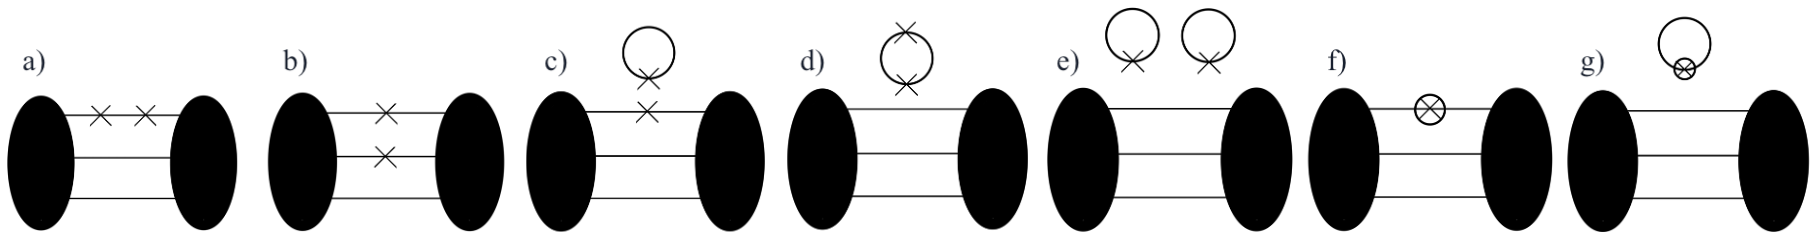
\includegraphics[width=15cm]{figures/diagrams.png}
  \caption{Relevant diagram contributions to the neutron electric polarizability. Note that the 
  crosses indicate the interaction vertices; linear in the external field interactions are represented with crosses, while the quadratic in the field interaction are represented by circles.}
  \label{fig:diagrams}
\end{figure}
In the case of a time-independent Hamiltonian that depends on the electric field
$E$ and gauge field $A$, which are considered to be two arbitrarily small parameters,
projecting onto unpolarized, zero-momentum neutrons, the two-point function
exhibits an exponential behavior at a large time:
\begin{equation}
G(p=0,t)=\sum_{\overrightarrow y}Tr\left(\frac{1+\gamma_0}{2}\langle N(y)\overline N(x)\rangle\right)\
\overset{t\rightarrow \infty}{\longrightarrow} W\exp(-mt)
\end{equation}
Expanding in $A$ and $E$, the overlap between the neutron source and the
ground state $W$, and the neutron mass $m$ are written as
\begin{equation}
\begin{split}
W&=W_0+W^{(1)}(A,E)+W^{(2)}(A,E)+\cdots\\
m&=m_0+m^{(2)}(A,E)+\cdots
\end{split}
\end{equation}
The second-order term in $A$ and $E$ in the neutron two-point function
is written as
\begin{equation}
G^{(2)}(p=0,t)\overset{t\rightarrow \infty}{\longrightarrow}W_0\exp(-m_0t)\left(\frac{W^{(2)}(A,E)}{W_0}-m^{(2)(A,E)t}\right)
\end{equation}
and, thus, the neutron mass shift $m^{(2)}$ can be obtained from the temporal slope of the 
correlator ratio, defined as
\begin{equation}
R_2(t)=\frac{G^{(2)}(p=0,t)}{G^{(0)}(p=0,t)}
\label{ratios}
\end{equation}
